\chapter{Methods}\label{chap:methods}
In this chapter, we discuss the methodology employed to develop a robust system that unifies the extraction of metadata from both article headers and references, regardless of the language in which they are written, English or German. We present our conceptual framework (Section~\ref{sec:conceptual_framework}), where we discuss our ideas and strategies aimed at addressing the research problems and how we want to solve them.\\
The chapter includes a detailed explanation of the datasets we annotated (Section~\ref{sec:methods_datasets}) and the thought process behind their creation. We discuss our intentions and considerations that guided us in assembling datasets that represent the problem domain and enable the training and evaluation of our models.\\
Furthermore, we provide insights into the models (Section~\ref{sec:methods_models}) we employed to accomplish our task of extracting metadata from scholarly literature.

\section{Conceptual Framework}\label{sec:conceptual_framework}
Upon conducting an extensive examination of available literature, software applications, and datasets related to our specific problems, we developed our conceptual framework. Our system's construction is predominantly inspired by well-regarded, peer-reviewed publications and established open-source software, namely EXParser, GROBID, CERMINE, and ParsCit. It is evident that each of these approaches employs a cascade of independently trained ML models or a combination of heuristics and ML techniques. The sequential nature of this approach introduces the risk of error propagation to downstream models and amplifies the presence of noisy or faulty input data with each passing layer.\\
However, in observing the benefits of a modular system, we found that it allows for greater flexibility in interchanging models and adapting training data as required. Consequently, we concluded that a modular system appears to be the most suitable choice. Nevertheless, we aimed to constrain the maximum depth of sequential models to minimize the propagation of uncertainty.\\
In Chapter~\ref{chap:background}, we investigated the current state-of-the-art models in the field of Natural Language Processing (NLP), with a focus on tasks related to multilingual document understanding, cross-lingual classification, and sequence labeling. Among the models we selected for utilization and testing are mBERT and XLM-RoBERTa, which are multilingual text-based models, capable of handling various languages and tasks. Additionally, we aim to incorporate LayoutXLM, a state-of-the-art multilingual model that not only considers text but also incorporates layout and visual information from documents, providing a comprehensive approach to document understanding. As a baseline comparison, we will include a CRF model, a widely used approach in related research as we discussed in Chapter~\ref{chap:related}.

\subsection{Document Segmentation Model}\label{sec:roadmap_docseg}
Our root model must possess the capability to identify relevant sections within a document, hence referred to as the Document Segmentation Model. As demonstrated by Rizvi et al.~\cite{rizvi2020hybrid}, visual information from scans can be effectively utilized for document segmentation. Therefore, we aimed to incorporate visual information into our model as well. Furthermore, our model must be able to handle both English and German corpora effectively. It should demonstrate robustness and accuracy in processing documents in both languages.\\
Considering the requirements for handling multimodal data and the utilization of visual information along with text in both English and German languages, we utilized LayoutXLM as our Document Segmentation Model for this processing step and formulated the following requirements for our Document Segmentation Dataset:
\begin{itemize}
    \item \textbf{Historical Literature:} The \textit{GEOcite} corpus consists of articles published over a period of 70 years. Ever changing citation styles, document layouts, and even vocabulary needs to be reflected in our data.
    \item \textbf{Data Representation:} As we want to employ a Multimodal Model, we need our data presented in various formats, encompassing textual content, corresponding layout information, and as digital images.
    \item \textbf{Robustness:} We want to employ a token-based sequence-to-sequence model instead of a line-based approach to account for possible errors of the OCR layout system. An example of this occurrence can be seen in Figure~\ref{fig:layout_error}.
    \item \textbf{Multilingual:} The data should consist of documents written in English and German.
    \item \textbf{Labels:} We need a minimum of two labels, one indicating header metadata and another for reference metadata. We prefer the labels to be as fine-grained as possible for an optimal extraction process.
\end{itemize}

\begin{figure}[!ht]
    \centering
    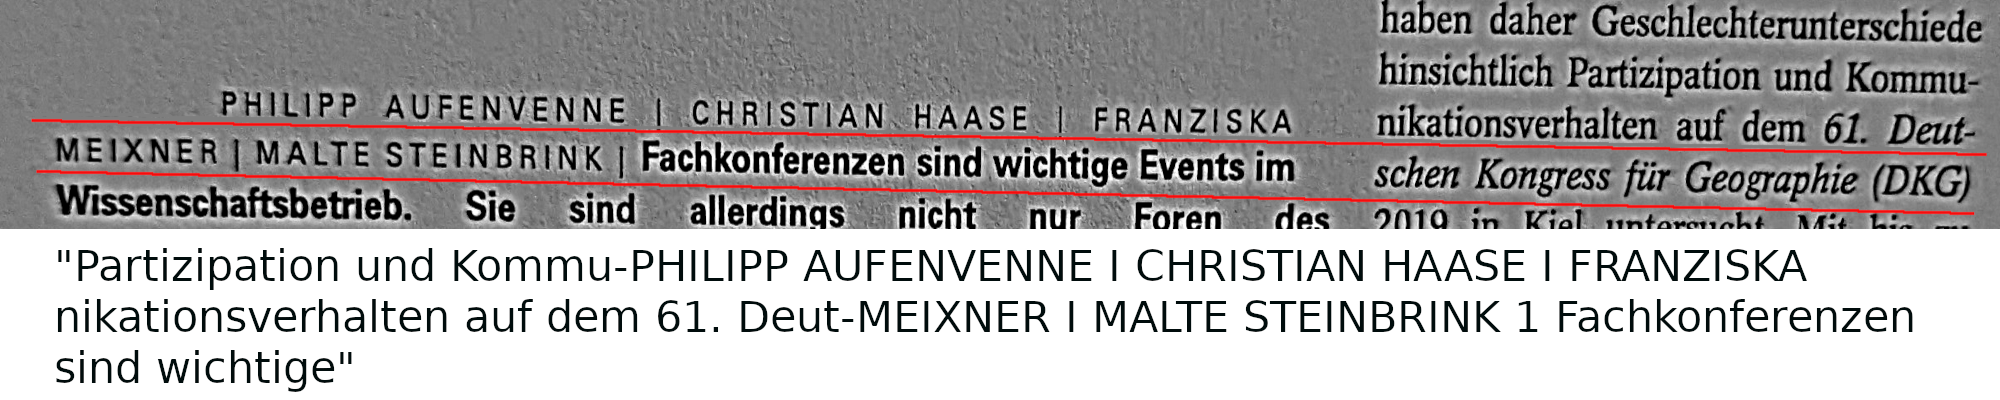
\includegraphics[width=1.0\linewidth]{images/layout_error.png}
    \caption{An example, where the layout detection of an OCR system fails. The upper part shows the detected layout, and the lower part shows the extracted text, complicating an extraction of article authors.}
    \label{fig:layout_error}
\end{figure}

We decided to utilize the DocBank dataset as the foundation for our Document Segmentation Dataset, fulfilling our requirements for robustness, data representation, and labels. To meet the historical literature and multilingual needs, we resolved to combine the DocBank dataset with an annotated dataset from the GEOcite analog corpus. Our annotated dataset was created with the intention of ensuring compatibility with the DocBank dataset in terms of output files (image, text, and layout information), format (e.g., normalized bounding boxes), and consistency of labeled data. This concatenation created a comprehensive dataset that aligns with all our requirements for fine-tuning the LayoutXLM model.

\subsection{Reference Parser Model}\label{sec:roadmap_reference_parser}
Our Document Segmentation Dataset is structured with references represented solely as word-level tokens, lacking any information about reference segments. Consequently, extracting metadata from references necessitates the use two separate models, one for reference segmentation and another for parsing the extracted reference strings.\\
To comply with our formulated robustness constraints and limit the depth of sequentially arranged models, we favored a unified approach, utilizing a single model capable in both reference segmentation and parsing. To achieve this, we fine-tuned an XML-RoBERTa model, augmented with a custom multi-output classification layer.\\
After thoroughly considering these aspects, we established the requisites for our Reference Parser Dataset:

\begin{itemize}
    \item \textbf{Domain:} The reference data in our dataset should be relevant to the domain of our corpus, particularly pertaining to the field of Geography. It should encompass specific aspects unique to the field, such as journal names and certain citation habits commonly found in Geography, such as references to local literature and newspapers.
    \item \textbf{Robustness:} Our reference strings should contain noise during training to enable the development of a robust system. By exposing the model to noisy reference data, it acquires the capacity to recover in case of errors induced from our upstream model. This deliberate inclusion of noise ensures that our parser model can withstand real-world challenges and inaccuracies, by enhancing its ability to handle variations and uncertainties in reference data.
    \item \textbf{Labels:} To support our multi-output model, we need two types of labels: a binary class to indicate whether a token marks the start of a new reference, and token-level labels for entities such as authors, titles, and journals. In addition, we need information about the start and end for each label, as they may span over multiple token.
\end{itemize}

We note, that the same requirements of \textbf{Multilingual} and \textbf{Historical Literature} as formulated in Section~\ref{sec:roadmap_docseg} also apply for this dataset. After analyzing our stated considerations, we decided to use the EXCite dataset as basis for our Reference Parser Dataset.\\
The suggested dataset utilizes a multilingual corpus and contains all the required labels. However, it does not fully meet our criteria as it includes modern Social Science articles from a broader domain, rather than from the domain of Geography itself. Furthermore, the GEOcite dataset does not encompass historical literature, which was formulated as another key requirement.\\
Given these considerations, we determined that the GEOcite dataset alone is not suitable as the basis for our Reference Parser Dataset and decided to address these limitations by annotating selected documents from our corpus and subsequently combining them with the GEOcite dataset. By doing so, we aimed to develop a comprehensive and domain-specific dataset that encompasses historical literature and fulfills all of our requirements for a sufficient Reference Parser Dataset.

\subsection{Author Parser Model}
The tokens labeled as authors from our Document Segmentation Model may also contain affiliations of the authors. Establishing citation networks relies heavily on accurately identifying the names of authors in scientific articles to link them with cited authors.\\
To accomplish this, we treat the task as a classical Named Entity Recognition (NER) problem, seeking to locate all persons mentioned in a block of text. We want to test the capabilities of mBERT, XLM-RoBERTa, and a CRF model on this task. As a result, we have formulated the following requirements for our dataset:

\begin{itemize}
    \item \textbf{Multilingual:} We want to account for language specific names and potential linguistic characteristics such as the French circumflex
    \item \textbf{Robustness:} The context in which we want to identify entities within our text block is highly constrained. To accommodate this limitation, our model should be trained on text snippets with restricted context, specifically avoiding long texts.
    \item \textbf{Labels:} We at least require a label to identify a person. However, we welcome additional labels such as organization or location, as they could potentially provide valuable information to further narrow down the author of an article.
\end{itemize}

The decision to use the WikiANN dataset as our Author Parser Dataset was driven by its unique advantages, which align well with our goals. The dataset offers a multilingual corpus, encompassing text snippets from various languages, making it suitable for evaluating the performance of our Author Parser Model on different language contexts.

\section{Datasets}\label{sec:methods_datasets}
In this section, we provide a detailed account of the methods we employed to create the datasets essential for training our models. We explore the technical aspects of the data generation process, illustrating the techniques utilized to ensure the datasets' quality and relevance. Furthermore, we address the challenges encountered during the dataset creation, discussing how we tackled various issues to achieve a comprehensive and robust training foundation for our models.

\subsection{Document Segmentation Dataset}\label{sec:document_segmentation_dataset}
Here, we present the creation process of our Document Segmentation Dataset, which serves as the foundation for training and testing our Document Segmentation Model. We outline the steps taken to obtain the data from two key sources: the GEOcite corpus and the DocBank corpus.

\subsubsection{GEOcite Corpus}
Due to the non-uniform distribution of articles across publication years in our corpus, we decided to employ a stratified sampling approach to gather the required documents. To achieve this, we divided the publication years into bins, each spanning 5 years, starting from the year 1949 until the present year. Subsequently, we sampled approximately 400 articles, ensuring an equal representation from each bin. By employing this stratified sampling method, we aim to create a dataset that is representative of the entire time span covered by our research while maintaining a balanced distribution of articles across different publication years.\\
It is our assumption that pages, with little or no information relevant to our research, would be over-represented in our dataset, since relevant metadata is expected to reside at the beginning and end of an article. With the median number of pages per article amounting to 8 pages, we expect that a considerable portion of content within each article may not directly contribute to our research objectives.\\
To address this issue, we classified the pages of an article into three distinct categories: a header page, identified by the presence of an author and title; a reference page, denoted by the presence of a reference; and a content page, recognized by the absence of author, title, and reference.\\
Next, we proceeded with the selection process, focusing on the first page of each document to extract its header page. For the identification of reference pages, we conducted a manual examination, marking all pages containing references. To ensure a balanced dataset, we sampled an equal number of pages from the reference pages, mirroring the number of header pages.\\
We further sampled an equivalent number of content pages from those that were neither designated as header nor reference pages. This comprehensive approach yielded a total of 1,365 pages, collectively forming our dataset, representative equally of the header, reference, and content pages.\\
Finally, we extracted words and bounding boxes from each page and used them to create digital images representing each page within our sample. To enhance the robustness of our overall system, we made the deliberate choice to retain irregularities and errors introduced by the OCR process. By preserving these imperfections, our system can adapt and handle real-world scenarios where OCR inaccuracies are common.\\

The annotation process for the sample was conducted using the annotation tool DataTurks~\cite{dataturks}. To ensure accuracy and consistency of our labeled data, we prepared an extensive annotation guide, documented in Appendix~\ref{chap:appendix_annotation}. This guide serves as a comprehensive reference for annotators, detailing the principles, rules, and criteria we established to achieve a well-structured and cleanly labeled dataset.\\
To streamline the annotation process for annotators, we have implemented measures for more accessibility and convenience. In addition to offering the textual representation of our sample, we provide access to PDFs and images of pages via a web server. This enables annotators to easily navigate and comprehend the context of the data they are annotating.\\

After the annotation process, we match the token labels with the corresponding token and bounding boxes. To ensure consistency with the DocBank dataset, we normalized the bounding boxes by following their proposed format, which closely resembles the format used in the MS COCO dataset~\cite{lin2014microsoft}. Here we denote coordinates of the rectangle using a tuple $(x_0, y_0, x_1, y_1)$, where $(x_0, y_0)$ corresponds to the location of the upper left corner in the bounding box, and $(x_1, y_1)$ represents the position of the lower right corner. To account for variations in resolution across transmitted images or PDFs, we employ min-max normalization to rescale the pixel values of the bounding boxes.
\begin{equation}
    x' = a + \frac{(x - \min{x})(b - a)}{\max{x} - \min{x}}
\end{equation}
This process ensures that the coordinates of the bounding boxes are adjusted to fall within a specified range of values, denoted as $[a, b]$, where $a = 0$, $b = 1000$.

\begin{table}[!ht]
	\centering
	\begin{tabular}{l|l|l|l|l|l|l|l|l|l|l}
        \textbf{Index} & \textbf{0} & \textbf{1} & \textbf{2} & \textbf{3} & \textbf{4} & \textbf{5} & \textbf{6} & \textbf{7} & \textbf{8} & \textbf{9} \\ \hline
        Content & token & $x_0$ & $y_0$ & $x_1$ & $y_1$ & R & G & B & font name & label
    \end{tabular}
	\caption{An overview about the data structure and contained layout information of the DocBank CSV file. $x_0$, $y_0$, $x_1$, and $y_1$ span the bounding box, R, G, and B yield the font color of a token.}
	\label{tab:docbank_data}
\end{table}

We saved our transformed sample as CSV files, following the same structure as the DocBank dataset, with the exception of the omitted features font and text color. Additionally, each CSV file is accompanied by a resized image with a resolution of 244 x 244 pixels. For reference, Table~\ref{tab:docbank_data} provides an overview of the data structure used in the DocBank dataset, aiding in understanding the organization and content of our dataset.\\
For testing the performance of our Document Segmentation Model, we set aside 10\% of our sampled data to create a separate test set. A comprehensive breakdown of the composition of the resulting GEOcite portion of our dataset can be examined in Table~\ref{tab:dataset_docseg_geocite}. It provides detailed insights into the distribution of different labels across the training and test set of our dataset.

\begin{table}[!ht]
\centering
\begin{tabular}{l|llllll|}
\cline{2-7}
\multicolumn{1}{c|}{}                & \multicolumn{6}{c|}{Document Segmentation Dataset - GEOcite Corpus}                                                                                                                                                                                                                                                                                                                 \\ \hline
\multicolumn{1}{|l|}{\textbf{label}} & \multicolumn{1}{l|}{\cellcolor[HTML]{DAE8FC}\textbf{train}} & \multicolumn{1}{l|}{\cellcolor[HTML]{EFEFEF}\textbf{}} & \multicolumn{1}{l|}{\cellcolor[HTML]{DAE8FC}\textbf{test}} & \multicolumn{1}{l|}{\cellcolor[HTML]{EFEFEF}\textbf{}} & \multicolumn{1}{l|}{\cellcolor[HTML]{DAE8FC}\textbf{total}} & \cellcolor[HTML]{EFEFEF}\textbf{} \\ \hline
\multicolumn{1}{|l|}{abstract}       & \multicolumn{1}{l|}{\cellcolor[HTML]{DAE8FC}35,070}         & \multicolumn{1}{l|}{\cellcolor[HTML]{EFEFEF}5.32\%}    & \multicolumn{1}{l|}{\cellcolor[HTML]{DAE8FC}5,473}         & \multicolumn{1}{l|}{\cellcolor[HTML]{EFEFEF}8.21\%}    & \multicolumn{1}{l|}{\cellcolor[HTML]{DAE8FC}40,543}         & \cellcolor[HTML]{EFEFEF}5.58\%    \\ \hline
\multicolumn{1}{|l|}{author}         & \multicolumn{1}{l|}{\cellcolor[HTML]{DAE8FC}2,347}          & \multicolumn{1}{l|}{\cellcolor[HTML]{EFEFEF}0.36\%}    & \multicolumn{1}{l|}{\cellcolor[HTML]{DAE8FC}256}           & \multicolumn{1}{l|}{\cellcolor[HTML]{EFEFEF}0.38\%}    & \multicolumn{1}{l|}{\cellcolor[HTML]{DAE8FC}2,603}          & \cellcolor[HTML]{EFEFEF}0.36\%    \\ \hline
\multicolumn{1}{|l|}{caption}        & \multicolumn{1}{l|}{\cellcolor[HTML]{DAE8FC}6,901}          & \multicolumn{1}{l|}{\cellcolor[HTML]{EFEFEF}1.05\%}    & \multicolumn{1}{l|}{\cellcolor[HTML]{DAE8FC}706}           & \multicolumn{1}{l|}{\cellcolor[HTML]{EFEFEF}1.06\%}    & \multicolumn{1}{l|}{\cellcolor[HTML]{DAE8FC}7,607}          & \cellcolor[HTML]{EFEFEF}1.05\%    \\ \hline
\multicolumn{1}{|l|}{equation}       & \multicolumn{1}{l|}{\cellcolor[HTML]{DAE8FC}31}             & \multicolumn{1}{l|}{\cellcolor[HTML]{EFEFEF}0.01\%}    & \multicolumn{1}{l|}{\cellcolor[HTML]{DAE8FC}0}             & \multicolumn{1}{l|}{\cellcolor[HTML]{EFEFEF}0\%}       & \multicolumn{1}{l|}{\cellcolor[HTML]{DAE8FC}31}             & \cellcolor[HTML]{EFEFEF}0.01\%    \\ \hline
\multicolumn{1}{|l|}{figure}         & \multicolumn{1}{l|}{\cellcolor[HTML]{DAE8FC}5,587}          & \multicolumn{1}{l|}{\cellcolor[HTML]{EFEFEF}0.85\%}    & \multicolumn{1}{l|}{\cellcolor[HTML]{DAE8FC}629}           & \multicolumn{1}{l|}{\cellcolor[HTML]{EFEFEF}0.94\%}    & \multicolumn{1}{l|}{\cellcolor[HTML]{DAE8FC}6,216}          & \cellcolor[HTML]{EFEFEF}0.86\%    \\ \hline
\multicolumn{1}{|l|}{footer}         & \multicolumn{1}{l|}{\cellcolor[HTML]{DAE8FC}36,008}         & \multicolumn{1}{l|}{\cellcolor[HTML]{EFEFEF}5.47\%}    & \multicolumn{1}{l|}{\cellcolor[HTML]{DAE8FC}4,270}         & \multicolumn{1}{l|}{\cellcolor[HTML]{EFEFEF}6.4\%}     & \multicolumn{1}{l|}{\cellcolor[HTML]{DAE8FC}40,278}         & \cellcolor[HTML]{EFEFEF}5.55\%    \\ \hline
\multicolumn{1}{|l|}{paragraph}      & \multicolumn{1}{l|}{\cellcolor[HTML]{DAE8FC}410,715}        & \multicolumn{1}{l|}{\cellcolor[HTML]{EFEFEF}62.36\%}   & \multicolumn{1}{l|}{\cellcolor[HTML]{DAE8FC}40,314}        & \multicolumn{1}{l|}{\cellcolor[HTML]{EFEFEF}60.45\%}   & \multicolumn{1}{l|}{\cellcolor[HTML]{DAE8FC}451,029}        & \cellcolor[HTML]{EFEFEF}62.18\%   \\ \hline
\multicolumn{1}{|l|}{reference}      & \multicolumn{1}{l|}{\cellcolor[HTML]{DAE8FC}142,033}        & \multicolumn{1}{l|}{\cellcolor[HTML]{EFEFEF}21.56\%}   & \multicolumn{1}{l|}{\cellcolor[HTML]{DAE8FC}13,334}        & \multicolumn{1}{l|}{\cellcolor[HTML]{EFEFEF}20\%}      & \multicolumn{1}{l|}{\cellcolor[HTML]{DAE8FC}155,367}        & \cellcolor[HTML]{EFEFEF}21.42\%   \\ \hline
\multicolumn{1}{|l|}{section}        & \multicolumn{1}{l|}{\cellcolor[HTML]{DAE8FC}4,427}          & \multicolumn{1}{l|}{\cellcolor[HTML]{EFEFEF}0.67\%}    & \multicolumn{1}{l|}{\cellcolor[HTML]{DAE8FC}380}           & \multicolumn{1}{l|}{\cellcolor[HTML]{EFEFEF}0.57\%}    & \multicolumn{1}{l|}{\cellcolor[HTML]{DAE8FC}4,807}          & \cellcolor[HTML]{EFEFEF}0.66\%    \\ \hline
\multicolumn{1}{|l|}{table}          & \multicolumn{1}{l|}{\cellcolor[HTML]{DAE8FC}10,123}         & \multicolumn{1}{l|}{\cellcolor[HTML]{EFEFEF}1.54\%}    & \multicolumn{1}{l|}{\cellcolor[HTML]{DAE8FC}692}           & \multicolumn{1}{l|}{\cellcolor[HTML]{EFEFEF}1.04\%}    & \multicolumn{1}{l|}{\cellcolor[HTML]{DAE8FC}10,815}         & \cellcolor[HTML]{EFEFEF}1.49\%    \\ \hline
\multicolumn{1}{|l|}{title}          & \multicolumn{1}{l|}{\cellcolor[HTML]{DAE8FC}5,387}          & \multicolumn{1}{l|}{\cellcolor[HTML]{EFEFEF}0.82\%}    & \multicolumn{1}{l|}{\cellcolor[HTML]{DAE8FC}638}           & \multicolumn{1}{l|}{\cellcolor[HTML]{EFEFEF}0.96\%}    & \multicolumn{1}{l|}{\cellcolor[HTML]{DAE8FC}6,025}          & \cellcolor[HTML]{EFEFEF}0.83\%    \\ \hline
\end{tabular}
\caption{The composition and amount of word-level token of the GEOcite portion of the Document Segmentation Dataset.}
\label{tab:dataset_docseg_geocite}
\end{table}

\subsubsection{DocBank Corpus}

Due to the limited size of our self-annotated data in comparison to the extensive DocBank dataset, we exercised caution in utilizing only a small portion of pages from the latter to avoid significant oversampling. To further ensure a representative sample, we adopted a stratified sampling approach, similar to that employed in the creation of the GEOcite portion of our dataset.\\
In this sampling process, we again focused on three distinct categories: header pages, reference pages, and content pages. By analyzing the token labels, we determined that a header page must contain at least one author and title label, a reference page must contain at least one reference label, and a content page must have neither an author, title, nor reference label. Overall, we sampled 500 pages from within each category.\\
We further noticed, that the DocBank dataset, being automatically generated, contains a limited number of irregularities. Some examples include malformed images of articles, article pages with only a few tokens, and faulty text encoding for word tokens. Given the constrained size of our constructed dataset, we aimed to ensure the utmost quality of our data.\\
To achieve this, we conducted a thorough search of all sampled pages and identified those with irregularities. Subsequently, we removed the pages with such anomalies and replaced them with new instances from within their respective categories.\\
Similarly to the approach used for the GEOcite corpus, we allocated 10\% of our data as a dedicated test set for evaluation purposes. Table~\ref{tab:dataset_docseg_docbank} provides a detailed visualization of the distribution of word-level tokens and labels within our dataset.

\begin{table}[!ht]
\centering
\begin{tabular}{l|llllll|}
\cline{2-7}
\multicolumn{1}{c|}{}                & \multicolumn{6}{c|}{Document Segmentation Dataset - DocBank Corpus}                                                                                                                                                                                                                                                                                                                 \\ \hline
\multicolumn{1}{|l|}{\textbf{label}} & \multicolumn{1}{l|}{\cellcolor[HTML]{DAE8FC}\textbf{train}} & \multicolumn{1}{l|}{\cellcolor[HTML]{EFEFEF}\textbf{}} & \multicolumn{1}{l|}{\cellcolor[HTML]{DAE8FC}\textbf{test}} & \multicolumn{1}{l|}{\cellcolor[HTML]{EFEFEF}\textbf{}} & \multicolumn{1}{l|}{\cellcolor[HTML]{DAE8FC}\textbf{total}} & \cellcolor[HTML]{EFEFEF}\textbf{} \\ \hline
\multicolumn{1}{|l|}{abstract}       & \multicolumn{1}{l|}{\cellcolor[HTML]{DAE8FC}56,912}         & \multicolumn{1}{l|}{\cellcolor[HTML]{EFEFEF}7.55\%}    & \multicolumn{1}{l|}{\cellcolor[HTML]{DAE8FC}6,430}         & \multicolumn{1}{l|}{\cellcolor[HTML]{EFEFEF}7.42\%}    & \multicolumn{1}{l|}{\cellcolor[HTML]{DAE8FC}63,342}         & \cellcolor[HTML]{EFEFEF}7.53\%    \\ \hline
\multicolumn{1}{|l|}{author}         & \multicolumn{1}{l|}{\cellcolor[HTML]{DAE8FC}11,318}         & \multicolumn{1}{l|}{\cellcolor[HTML]{EFEFEF}1.5\%}     & \multicolumn{1}{l|}{\cellcolor[HTML]{DAE8FC}2,136}         & \multicolumn{1}{l|}{\cellcolor[HTML]{EFEFEF}2.46\%}    & \multicolumn{1}{l|}{\cellcolor[HTML]{DAE8FC}13,454}         & \cellcolor[HTML]{EFEFEF}1.6\%     \\ \hline
\multicolumn{1}{|l|}{caption}        & \multicolumn{1}{l|}{\cellcolor[HTML]{DAE8FC}13,414}         & \multicolumn{1}{l|}{\cellcolor[HTML]{EFEFEF}1.78\%}    & \multicolumn{1}{l|}{\cellcolor[HTML]{DAE8FC}1,661}         & \multicolumn{1}{l|}{\cellcolor[HTML]{EFEFEF}1.92\%}    & \multicolumn{1}{l|}{\cellcolor[HTML]{DAE8FC}15,075}         & \cellcolor[HTML]{EFEFEF}1.79\%    \\ \hline
\multicolumn{1}{|l|}{equation}       & \multicolumn{1}{l|}{\cellcolor[HTML]{DAE8FC}28,618}         & \multicolumn{1}{l|}{\cellcolor[HTML]{EFEFEF}3.79\%}    & \multicolumn{1}{l|}{\cellcolor[HTML]{DAE8FC}1,656}         & \multicolumn{1}{l|}{\cellcolor[HTML]{EFEFEF}1.91\%}    & \multicolumn{1}{l|}{\cellcolor[HTML]{DAE8FC}30,274}         & \cellcolor[HTML]{EFEFEF}3.6\%     \\ \hline
\multicolumn{1}{|l|}{figure}         & \multicolumn{1}{l|}{\cellcolor[HTML]{DAE8FC}15,311}         & \multicolumn{1}{l|}{\cellcolor[HTML]{EFEFEF}2.03\%}    & \multicolumn{1}{l|}{\cellcolor[HTML]{DAE8FC}67}            & \multicolumn{1}{l|}{\cellcolor[HTML]{EFEFEF}0.08\%}    & \multicolumn{1}{l|}{\cellcolor[HTML]{DAE8FC}15,378}         & \cellcolor[HTML]{EFEFEF}1.83\%    \\ \hline
\multicolumn{1}{|l|}{footer}         & \multicolumn{1}{l|}{\cellcolor[HTML]{DAE8FC}4,783}          & \multicolumn{1}{l|}{\cellcolor[HTML]{EFEFEF}0.63\%}    & \multicolumn{1}{l|}{\cellcolor[HTML]{DAE8FC}576}           & \multicolumn{1}{l|}{\cellcolor[HTML]{EFEFEF}0.66\%}    & \multicolumn{1}{l|}{\cellcolor[HTML]{DAE8FC}5,359}          & \cellcolor[HTML]{EFEFEF}0.64\%    \\ \hline
\multicolumn{1}{|l|}{paragraph}      & \multicolumn{1}{l|}{\cellcolor[HTML]{DAE8FC}465,221}        & \multicolumn{1}{l|}{\cellcolor[HTML]{EFEFEF}61.7\%}    & \multicolumn{1}{l|}{\cellcolor[HTML]{DAE8FC}55,610}        & \multicolumn{1}{l|}{\cellcolor[HTML]{EFEFEF}64.2\%}    & \multicolumn{1}{l|}{\cellcolor[HTML]{DAE8FC}520,831}        & \cellcolor[HTML]{EFEFEF}61.96\%   \\ \hline
\multicolumn{1}{|l|}{reference}      & \multicolumn{1}{l|}{\cellcolor[HTML]{DAE8FC}146,663}        & \multicolumn{1}{l|}{\cellcolor[HTML]{EFEFEF}19.45\%}   & \multicolumn{1}{l|}{\cellcolor[HTML]{DAE8FC}17,462}        & \multicolumn{1}{l|}{\cellcolor[HTML]{EFEFEF}20.16\%}   & \multicolumn{1}{l|}{\cellcolor[HTML]{DAE8FC}164,125}        & \cellcolor[HTML]{EFEFEF}19.53\%   \\ \hline
\multicolumn{1}{|l|}{section}        & \multicolumn{1}{l|}{\cellcolor[HTML]{DAE8FC}3,990}          & \multicolumn{1}{l|}{\cellcolor[HTML]{EFEFEF}0.53\%}    & \multicolumn{1}{l|}{\cellcolor[HTML]{DAE8FC}402}           & \multicolumn{1}{l|}{\cellcolor[HTML]{EFEFEF}0.46\%}    & \multicolumn{1}{l|}{\cellcolor[HTML]{DAE8FC}4,392}          & \cellcolor[HTML]{EFEFEF}0.52\%    \\ \hline
\multicolumn{1}{|l|}{table}          & \multicolumn{1}{l|}{\cellcolor[HTML]{DAE8FC}4,396}          & \multicolumn{1}{l|}{\cellcolor[HTML]{EFEFEF}0.58\%}    & \multicolumn{1}{l|}{\cellcolor[HTML]{DAE8FC}261}           & \multicolumn{1}{l|}{\cellcolor[HTML]{EFEFEF}0.3\%}     & \multicolumn{1}{l|}{\cellcolor[HTML]{DAE8FC}4,657}          & \cellcolor[HTML]{EFEFEF}0.55\%    \\ \hline
\multicolumn{1}{|l|}{title}          & \multicolumn{1}{l|}{\cellcolor[HTML]{DAE8FC}3,326}          & \multicolumn{1}{l|}{\cellcolor[HTML]{EFEFEF}0.44\%}    & \multicolumn{1}{l|}{\cellcolor[HTML]{DAE8FC}361}           & \multicolumn{1}{l|}{\cellcolor[HTML]{EFEFEF}0.42\%}    & \multicolumn{1}{l|}{\cellcolor[HTML]{DAE8FC}3,687}          & \cellcolor[HTML]{EFEFEF}0.43\%    \\ \hline
\end{tabular}
\caption{The composition and amount of word-level token of the DocBank portion of the Document Segmentation Dataset.}
\label{tab:dataset_docseg_docbank}
\end{table}

Finally, the two portions of the dataset, the DocBank corpus and the self-annotated data from the GEOcite corpus, are joined to create the Document Segmentation Dataset. This unified dataset comprises resized images, along with corresponding tokens and bounding boxes. In total, the dataset contains 2,579 instances for training and 286 instances for testing.

\subsection{Reference Parser Dataset}
The EXCite dataset, which we use as foundation of the Reference Parser Dataset, contains one XML file per document, where each line in this document resembles one reference string. The different entities are enclosed with XML tags, resembling their label. Figure~\ref{fig:reference_xml} illustrates the exact structure of the EXCite dataset.\\
The existing split of the training and test sets in the EXCite dataset is conducted at the document level rather than considering the overall number of reference strings. While this approach may lead to an unbalanced distribution of training and test instances due to potential sampling variations, we made the decision to follow the same document-level split for our labeled data. This choice ensures that the ratio of training and test documents aligns with that of the EXCite dataset, enabling us to maintain a coherent dataset.

\begin{figure}[!ht]
    \centering
    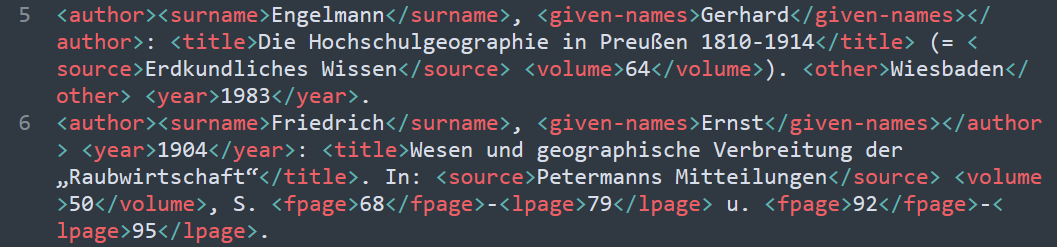
\includegraphics[width=0.95\linewidth]{images/example_reference_xml.png}
    \caption{The contents of an XML file from the GEOcite dataset.}
    \label{fig:reference_xml}
\end{figure}

As previously described in Section ~\ref{sec:document_segmentation_dataset}, we employed a stratified sampling approach based on the historic distribution of articles. This method yielded a collection of 188 documents.\\
Subsequently, we extracted the text layer from the obtained PDF files to prepare the data for annotation and decided, following our principle of robustness, to keep potential errors induced by the OCR process.\\

To accomplish the annotation process, we utilized the EXRef-Identifier, an annotation tool that is part of the EXannotator incorporated in the EXCITE toolchain, integrated in the EXCITE toolchain.\\
In the initial annotation step, we focused on extracting and segmenting references from our sample literature. The output files generated from this process were subsequently fed into a second annotation tool called EXRef-Segmentation. This second tool was utilized to identify and annotate specific entities within each reference string, including author names, titles, publication dates, and journal information.\\
This process resulted in 5,073 annotated reference strings from the GEOcite corpus, totaling the cumulative amount of reference strings to 17,569.\\

Next, we extracted token-strings and converted XML-tags of each entity to IOB2-tags. New lines indicate a new reference, which we use to label the first token-string of each line as beginning of a reference, all other token-strings are labeled as intermediate in this regard.\\
Note, that we do not yet use word-level token at this step, as the further tokenization process is dependent on the used tokenizer and employed model. In Table~\ref{tab:reference_segmented}, we present a comprehensive illustration of the resulting token-strings and their corresponding labels.\\
We will explain in detail, how we construct our atomic training and test instances, tokenization, and how this approach will aid in a robust training in Section~\ref{sec:component_ref_parser}.

\begin{table}[!ht]
    \centering
    \begin{tabular}{|l|l|l|l|}
        \hline
        \textbf{token-string} & \textbf{entity IOB} & \textbf{entity label} & \textbf{segment IOB} \\ \hline \hline
        Engelmann & B & author & B \\ \hline
        ,  & I & author & I \\ \hline
        Gerhard & I & author & I \\ \hline
        : & O & O & I \\ \hline
        Die Hochschulgeo(...) & B & title & I \\ \hline
        ( & O & O & I \\ \hline
        Erdkundliches Wissen & B & source & I \\ \hline
        , & O & O & I \\ \hline
        64 & B & volume & I \\ \hline
        ). & O & O & I \\ \hline
        Wiesbaden & B & other & I \\ \hline
        , & O & O & I \\ \hline
        1983 & B & year & I \\ \hline
        . & O & O & I \\ \hline
    \end{tabular}
    \label{tab:reference_segmented}
    \caption{An exemplary structure of the Reference Parser Dataset. The \textit{entity IOB} and \textit{entity label} together form IOB-labels, e.g. B-author or I-author. The \textit{segment IOB} label indicates the beginning of a new reference.}
\end{table}

After generating the CSV files containing the token-strings and labels, we proceed to split them into training and test sets, ensuring the same training and test split ratio as the GEOcite dataset. By maintaining this consistency, the concatenation of the GEOcite documents and our self-annotated documents results in a combined total of 373 training documents and 50 test documents, forming the Reference Parser Dataset.\\
An overview of all employed labels of our datasets can be seen in Table~\ref{tab:datasets_label}.

\begin{table}[!ht]
	\centering
	\begin{tabularx}{\textwidth}{l|l|X}
        \textbf{Dataset} & \textbf{Model} & \textbf{Labels}\\ \hline
        DocBank & Document Segmentation & \textit{abstract, author, caption, date, equation, figure, footer, list, paragraph, reference, section, table, title}\\\hline
        EXCITE & Reference Parser & \textit{publisher, first page, last page, title, url, author, author surname, author given-name, volume, source, editor, identifier, year, issue, other}\\\hline
        WikiANN & Author Parser & \textit{person, organisation, location}\\ \hline
    \end{tabularx}
	\caption{The utilized datasets as foundations for our models and their class labels.}
	\label{tab:datasets_label}
\end{table}

\section{Component Models}\label{sec:methods_models}
In this section, we provide a detailed exposition of the proposed modular component models, which build the foundation of our overall system. We address the intricate aspects of our methodology, covering explicit training sample generation, tokenization techniques, selection of hyperparameters, and the overall process of each of our component models' training.

\subsection{Document Segmentation Model}\label{sec:doc_model}
Many large transformer models are limited in their maximum number of input tokens, due to the use of their self-attention mechanism~\cite{vaswani2017attention} to capture long-term dependencies between all inputs of a sequence~\cite{devlin2019bert,liu2019roberta,sanh2019distilbert}. The quadratic complexity of Transformers with respect to its input sequence length, forces most model architectures to fix the length of their input sequence~\cite{wang2020linformer}.\\
While this limitation is acceptable for some applications, such as document classification or sentiment analysis, where a section of a text might suffice, sequence-to-sequence problems require the whole input length.\\
The LayoutXLM model is also constrained by these limitations, but our focus lies on classifying the entire set of tokens in a document. This emphasis results from the observation that reference sections can sometimes begin in the lower part of an article. As a result, we cannot rely solely on fixed-length single instances per page during our model fine-tuning, as they may lead to the exclusion of crucial information present in the lower sections.\\
To overcome this challenge, we decided to slice our dataset into snippets, each consisting of the maximum allowed model length of 512 tokens. In order to avoid worst-case scenarios, where a document with, for example, 513 tokens would be split into two parts of 512 token and 1 token respectively, we adopted the strategy of dividing the token per document into equal-length parts.\\

Our bounding boxes were already normalized during the dataset creation. The extracted images have the correct dimensions, but we converted them to BGR images in the preprocessing phase for our model fine-tuning, since the visual backbone expects this byte-order of color channels.\\
The tokenization was conducted utilizing a SentencePiece tokenizer~\cite{kudo2018sentencepiece} using the byte-pair-encoding subword algorithm~\cite{sennrich2016neural}. To comply with the maximum length by our model, we used padding for input token sequences. Sequences that are shorter than the maximum length, were filled in with a special $<pad>$ token. The start and end of a sequence are marked with the special token $<s>$ and $</s>$.\\
Since the position embedding layer for bounding boxes is concatenated with the text embedding layer, LayoutXLM utilizes a special empty position embedding $box_{PAD}$ aligning with all special token of the text embedding layer.\\
In our approach, subwords were not individually labeled, and we assigned them the value of -100. This value is utilized by PyTorch during the loss calculation. When computing the loss, PyTorch ignores the weights of subwords with this assigned value, effectively excluding them from contributing to the loss calculation.\\
As evident in Table~\ref{tab:dataset_docseg_geocite} and Table~\ref{tab:dataset_docseg_docbank}, we observed a highly imbalanced distribution of word-level tokens in our dataset. For instance, the majority class \textit{'paragraph'} accounts for approximately 62\% of all word-level tokens. To address potential bias towards highly frequent classes, we designed a weight vector with weights inversely proportional to their class frequencies. These weights are utilized during our model training to appropriately scale the loss function, ensuring a more balanced learning process and fair treatment of all classes.\\
Our hyperparameters, which we are trying to tune are the
\begin{itemize}
    \item learning rate: one of three values $[1e-5, 5e-5, 1e-4]$
    \item batch size: one of two values $[4, 8]$
    \item warm-up ratio: one of two values $[0, 0.1]$
\end{itemize}

Due to the split of pages into multiple samples, we ended up with multiple training instances representing the same page. To address the risk of overfitting, we limited the maximum number of training epochs to 2.\\
We conducted a 5-fold cross-validation on our training set to find our optimal model parameters. The best hyperparameters were used to fine-tune the LayoutXLM model on our whole training set and evaluated against our test set. Due to the aforementioned class imbalances we evaluate our model using the F1-score.

\subsection{Reference Parser Model}\label{sec:component_ref_parser}
As highlighted in Section~\ref{sec:roadmap_reference_parser}, one of our key objectives was to train the Reference Parser Model in a robust manner. The model receives its input tokens from the Document Segmentation Model upstream, which might contain noisy data due to the challenges of OCR and document segmentation.\\
Through our research, we have found that most existing tools and approaches use individual reference strings as input for their respective parser models to extract the required metadata. However, we opted for a slightly different approach, by feeding multiple reference strings into our model to extract atomic label from a broader context.\\
The core concept behind our proposed method is to train the model using fixed-size snippets of composite reference strings originating from the same document. These snippets can contain multiple reference strings and begin and end at random positions within a reference string.\\
Our goal is to provide diverse and contextually rich input to the model, enabling it to recover from faulty input more easily and learn within its given context. By exposing the model to varied snippets, it gains a better understanding of reference string structures and can make more accurate metadata extraction decisions, even in the presence of noisy data.\\
To accommodate the model's requirement to predict two outputs, the atomic label and the token indicating the start of a new reference, we implemented a custom classification layer and adapted the loss function to incorporate both predictions during model training. We add two linear layers connected to the last hidden layer resembling the output sequence.\\
The new loss function is the sum of the cross entropy between the entity targets (author, title, year, etc.)   and binary cross entropy is defined as
\begin{equation}
    \ell(x,y) = \ell_A(x_A,y_A) + \alpha \cdot \ell_B(x_B, y_B)
\end{equation}
with
\begin{equation}
    \ell_A(x_A,y_A) = \{l_{A_{1}},...,l_{A_{N}}\}^T, l_{A_{n}} = -w_{y_{A_{n}}} log\frac{\exp(x_{A_{n,y_{n}}})}{\sum_{c=1}^{C}\exp(x_{A_{n,c}})}
\end{equation}
\begin{equation}
    \ell_B(x_B,y_B) = \{l_{B_{1}},...,l_{B_{N}}\}^T, l_{B_{n}} = -w_{B_{n}} [y_{B_{n}} \cdot \log x_{B_{n}} + (1 - y_{B_{n}}) \cdot \log(1 - x_{B_{n}})] 
\end{equation}

where $x$ is the input, $y$ is the target, $C$ is the number of classes, and $N$ spans the minibatch dimension.\\
$\ell_A(x_A,y_A)$ is the cross entropy loss of our entity targets (author, title, year, etc.) with its input $x_A$, target $y_A$, and weight $w_A$. $\ell_B(x_B,y_B)$ is the binary cross entropy loss indicating a new reference with its corresponding input $x_B$, target $y_B$, and weight $w_B$. $\alpha$ is a parameter in the range $[0,1]$ to adjust, for emphasising one of the two outputs.\\
Given that our Reference Parser Dataset comprises token-strings instead of word-level tokens, we further preprocessed and pretokenized our data. This pretokenization involved splitting tokens based on white-spaces, digits, and specific punctuation marks such as ".", ":", ",", ";", "/", "-", "(", and ")".\\
To ensure comprehensive evaluation, we generated training and testing slices from the pretokenized data. This resulted in 2,047 training slices and 247 test slices.\\
Since the model we fine-tune, XLM-RoBERTa, also utilizes SentencePiece for tokenization, the further tokenization process is similar as described in Section~\ref{sec:doc_model}. An exemplary slice of the final dataset used for fine-tuning and testing of our model can be seen in Table~\ref{tab:ref_parser_sliced_output}.

\begin{table}[!ht]
    \centering
    \begin{tabular}{|l|l|l|}
    \hline
        \textbf{Token} & \textbf{IOB entity} & \textbf{IOB reference} \\ \hline
        \_Baden & B-other & I-ref \\ \hline
        \_- & I-other & I-ref \\ \hline
        \_Baden & I-other & I-ref \\ \hline
        \_: & O & I-ref \\ \hline
        \_No & B-publisher & I-ref \\ \hline
        mos & -100 & I-ref \\ \hline
        \_. & O & I-ref \\ \hline
        \_Drake & B-author & B-ref \\ \hline
        \_W & I-author & I-ref \\ \hline
        \_. & I-author & I-ref \\ \hline
        \_J & I-author & I-ref \\ \hline
        \_. & I-author & I-ref \\ \hline
        \_( & O & I-ref \\ \hline
        \_2005 & B-year & I-ref \\ \hline
    \end{tabular}
    \caption{An example of a reference string slice, used for fine-tuning our Reference Parser Model.}
    \label{tab:ref_parser_sliced_output}
\end{table}

The hyperparameters we are fine-tuning
\begin{itemize}
    \item learning rate:  $[1e-5, 5e-5, 1e-4]$
    \item batch size: $[4, 8, 16]$
    \item epochs: $[1-3]$
\end{itemize}
were evaluated on a 5-fold crossvalidation. Afterwards we trained our model with the best performing parameters on our whole training set. As evaluation metric we used the proposed method, focusing on text chunking, introduced on the CoNLL-2000 shared task~\cite{tjong-kim-sang-buchholz-2000-introduction}.

\subsection{Author Parser Model}
In our analysis, we observed that certain journals commonly print author names in uppercase letters only, as evident in Figure~\ref{fig:layout_error}. However, depending on the tokenization algorithm used, this practice can result in significantly different representations of an author's name. For instance, the name \enquote{Aufenvenne} could be split into 'AU', '\#\#F', '\#\#EN', '\#\#VE', '\#\#N', '\#\#NE' as uppercase and 'auf', '\#\#en', '\#\#ven', '\#\#ne' as lowercase. This discrepancy may lead to completely different word embeddings.\\
Due to potential character misclassifications of the OCR system, such as between uppercase and lowercase 'I' characters, we made a deliberate decision to use an uncased multilingual BERT model. Despite uppercase letters being a strong indicator for identifying person names, opting for an uncased model allows for a more consistent and robust extraction of author names across all journals in our corpus.\\

We combined the four parts of the wikiAnn dataset by interleaving them, resulting in a unified training and test set of text sequences in German, English, French, and Spanish. For each language, we obtained 20,000 training samples and 10,000 test samples.\\
To preprocess the dataset, we tokenized it using a word-piece tokenizer and padded the input token sequences. For sequences shorter than the maximum length supported by our chosen BERT model, we used a special $[PAD]$ token to fill in the remaining positions. To indicate the start and end of each sequence, we used the special tokens $[CLS]$ and $[SEP]$, respectively.\\
As in our previous component models, subwords were not labeled.\\
The hyperparameters we are fine-tuning are
\begin{itemize}
    \item learning rate:  $[1e-5, 5e-5, 1e-4]$
    \item batch size: $[8, 16]$
    \item epochs: $[1-3]$
\end{itemize}
As in the previous models, we conducted a 5-fold cross-validation on our training set to find our optimal model parameters.

\section{Used Software and Tools}
We used the Annotation tools DataTurks~\cite{dataturks} and EXannotator~\cite{excite_toolchain} to generate the labels for our datasets. We further used the base LayoutXML~\cite{hug_layoutxlm}, base XML-RoBERTa~\cite{hug_xlmr}, multilingual uncased~\cite{hug_uncased_bert} and cased BERT~\cite{hug_cased_bert} models from the data science platform Hugging Face~\cite{wolf2019huggingface}.